\chapter{Hunt for BLAs : The Survey} \label{ch:Survey}

The foremost goal of the current study is to do a survey of BLAs over a large data-set and then estimate their contribution in the closure density of $\Omega_b$. In this chapter we describe our approach to carry out this exhaustive survey.

\section{Shortlisting the BLA candidates} \label{sec:BLA-candidates}

\citet{danforth-2016} have identified a total of 2611 absorber systems in their study of low redshift intergalactic medium. We need to find suitable candidates for our survey of BLAs from these 2611 absorbers.

We use two criterias to select BLA candidates for our survey. First, we look for broad Ly$\alpha$ lines in all the 2611 absorbers. For a Ly$\alpha$ line to be adjudged as `broad', we fix our threshold for \emph{b} value to be greater than 45 km s$^{-1}$ in the preliminary fitting done by \citet{danforth-2016}. Assuming a complete thermal broadening, $\emph{b}=45$ km s$^{-1}$ gives a temperature of $\approx 1.2 \times 10^5$ K, which lies in the lower ranges of the temperature of WHIM. By giving this constrain, we get 568 such systems in the complete data-set.

As discussed in section \ref{sec:WHIM-BLA}, multiple lines or contaminations from other lines can blend together to give rise to broad absorption features. In such cases, we need to carefully model these broad lines and confirm that these are actually tracing hot collisionally ionised gas phase so that they are indeed probing WHIM and not just cool photoionised phase. We need to perform ionisation modelling for it. To model the ionisation conditions of the absorber systems, we need metal ion column densities. So we search for systems showing metal line absorption in these 568 `broad' systems. We need at least three distinct metal ions (not lines) to better constrain the ionisation state of an absorber system. This sets our second criteria that there should be minimum of three metal ion absorption in the absorber systems. Upon putting this constrain, we get 29 systems having at least 3 distinct metal ions out of 568 already identified systems. Out of these 29 systems, we have already studied one of the absorber in chapter \ref{ch:PG0003}. Table \ref{tab:BLA-candidates} lists the lines of sight, redshift of the absorber and the ions detected in the systems these 29 identified BLA candidate absorber systems. Figure \ref{fig:metal-ions-hist} shows the distribution of different metal ions found in these 29 absorber systems. 


\begin{figure}
    \centering
    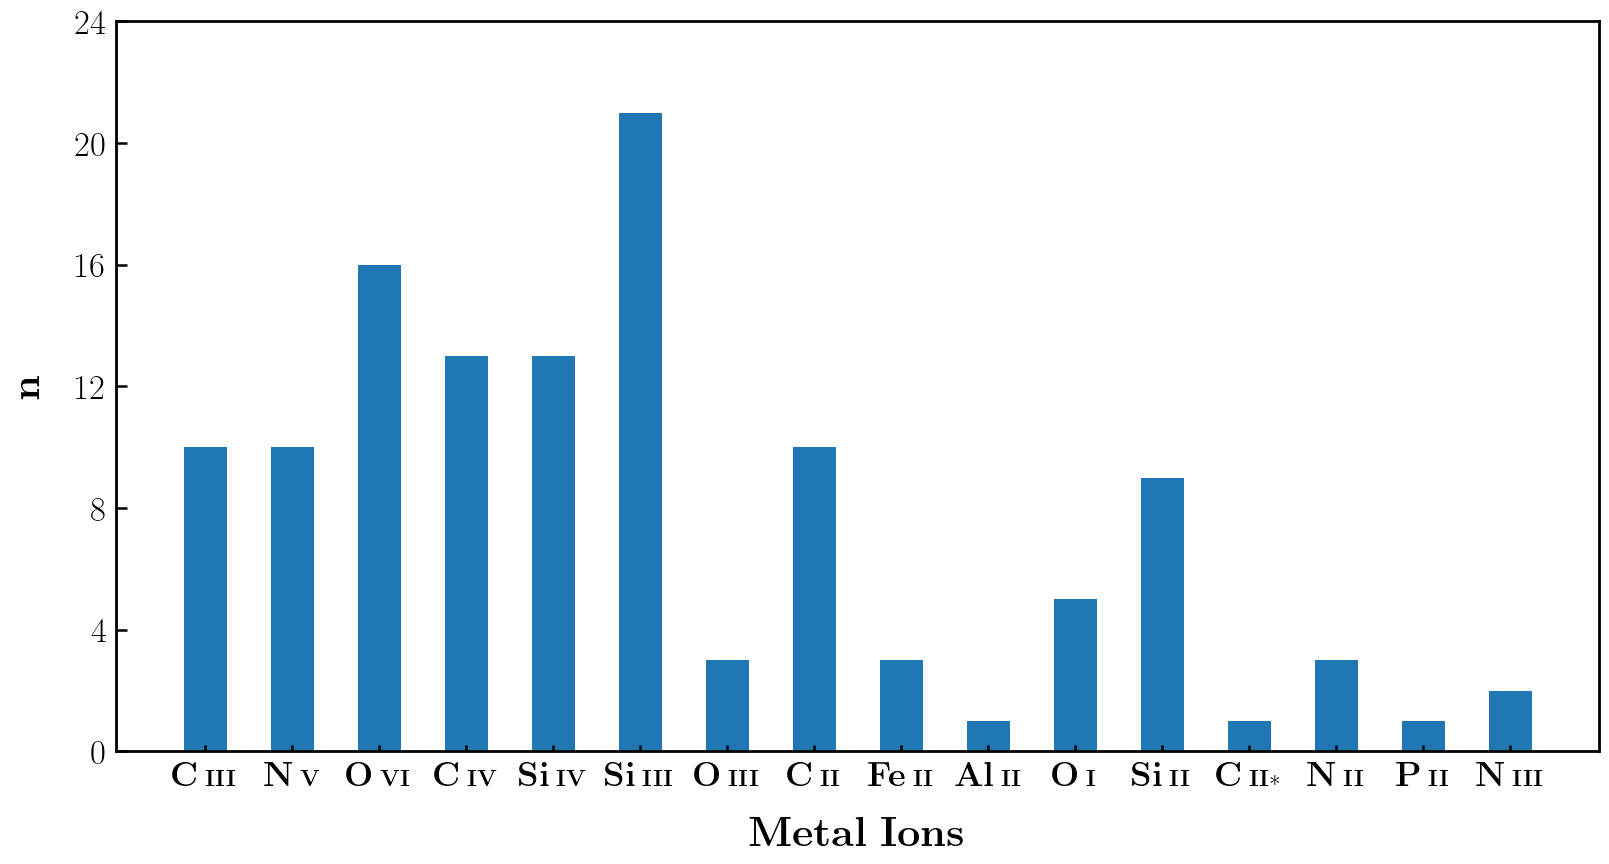
\includegraphics[width=\linewidth]{Figures/metal-ions.png}
    \caption{No. of different metal ions in all the 29 absorber systems.}
    \label{fig:metal-ions-hist}
\end{figure}


\begin{table}
\centering
\vspace{5mm}
\hspace*{-15mm}
    \begin{tabular}{cccc}
        \hline \hline
       \head{S. no.} & \head{Sight line} & \head{$\mathbf{z_{abs}}$} &  \head{Metal ions}
       \tabularnewline \hline  \tabularnewline
1    &    1ES 1553+113   &   0.187731   &  \ion{C}{iii}, \ion{O}{vi}, \ion{N}{v}   \\ 
2    &    3C 263   &   0.063275   &  \ion{C}{iv}, \ion{Si}{iii}, \ion{Si}{iv}   \\ 
3    &    3C 263   &   0.140754   &  \ion{C}{iv}, \ion{Si}{iii}, \ion{O}{vi}   \\ 
4    &    3C 57   &   0.077493   &  \ion{C}{iv}, \ion{Si}{iv}, \ion{N}{v}   \\ 
5    &    H 1821+643   &   0.170062   &  \ion{Si}{iii}, \ion{O}{vi}, \ion{N}{v}   \\ 
6    &    H 1821+643   &   0.224832   &  \ion{Si}{iii}, \ion{O}{vi}, \ion{C}{iii}   \\ 
7    &    HE 0056-3622   &   0.043318   &  \ion{C}{iv}, \ion{Si}{iii}, \ion{N}{v}   \\ 
8    &    PMN J1103-2329   &   0.003975   &  \ion{C}{iv}, \ion{Si}{iii}, \ion{Si}{iv}, \ion{N}{v}   \\ 
9    &    PG 0003+158   &   0.386094   &  \ion{C}{iii}, \ion{O}{vi}, \ion{O}{iii}, \ion{N}{v}   \\ 
10    &    PG 0003+158   &   0.347586   &  \ion{C}{ii}, \ion{C}{iii}, \ion{Si}{ii}, \ion{Si}{iii}, \ion{O}{vi}\\ 
11    &    PG 0003+158   &   0.421880   &  \ion{O}{vi}, \ion{O}{iii}, \ion{C}{iii}   \\ 
12    &    PG 0832+251   &   0.017520   &  \ion{C}{iv}, \ion{Si}{iv}, \ion{C}{ii*}, \ion{O}{i}, \ion{Si}{iii}, \ion{C}{ii}, \ion{Si}{ii}, \ion{Fe}{ii}, \ion{Al}{ii}, \ion{N}{v}   \\ 
13    &    PG 1116+215   &   0.138527   &  \ion{C}{iv}, \ion{Si}{iv}, \ion{N}{ii}, \ion{P}{ii}, \ion{Si}{iii}, \ion{Si}{ii}, \ion{C}{ii}, \ion{O}{vi}, \ion{N}{v}   \\ 
14    &    PG 1121+422   &   0.192434   &  \ion{Si}{iv}, \ion{C}{iii}, \ion{Si}{iii}, \ion{Si}{ii}, \ion{C}{ii}, \ion{O}{vi}   \\ 
15    &    PG 1216+069   &   0.006390   &  \ion{O}{i}, \ion{Si}{ii}, \ion{C}{ii}   \\ 
16    &    PG 1216+069   &   0.282195   &  \ion{Si}{iii}, \ion{O}{vi}, \ion{C}{iii}   \\ 
17    &    PG 1222+216   &   0.054491   &  \ion{C}{iv}, \ion{Si}{iii}, \ion{Si}{iv}   \\ 
18    &    PG 1222+216   &   0.378600   &  \ion{Si}{iii}, \ion{O}{vi}, \ion{O}{iii}, \ion{C}{iii}   \\ 
19    &    PG 1259+593   &   0.046107   &  \ion{C}{iv}, \ion{Si}{iii}, \ion{Si}{iv}   \\ 
20    &    PG 1424+240   &   0.146789   &  \ion{C}{iv}, \ion{Si}{iii}, \ion{O}{vi}, \ion{Si}{iv}   \\ 
21    &    PHL 1811   &   0.080837   &  \ion{C}{iv}, \ion{Si}{iv}, \ion{N}{ii}, \ion{O}{i}, \ion{Fe}{ii}, \ion{Si}{ii}, \ion{C}{ii}   \\ 
22    &    PKS 0405-123   &   0.167125   &  \ion{Si}{iv}, \ion{N}{ii}, \ion{C}{iii}, \ion{O}{i}, \ion{Si}{iii}, \ion{Si}{ii}, \ion{C}{ii}, \ion{O}{vi}, \ion{N}{iii}, \ion{N}{v}   \\ 
23    &    PKS 0637-752   &   0.161068   &  \ion{Si}{iii}, \ion{O}{vi}, \ion{N}{v}   \\  
24    &    PKS 0637-752   &   0.417573   &  \ion{Si}{iii}, \ion{O}{vi}, \ion{C}{iii}   \\ 
25    &    PKS 1302-102   &   0.094864   &  \ion{Si}{iii}, \ion{Si}{ii}, \ion{C}{ii}   \\ 
26    &    RX J0439.6-5311   &   0.005602   &  \ion{C}{iv}, \ion{Si}{iii}, \ion{Si}{iv}   \\ 
27    &    SDSS J135712.61+170444   &   0.097767   &  \ion{C}{iv}, \ion{Si}{iv}, \ion{Si}{iii}, \ion{C}{ii}, \ion{O}{vi}   \\ 
28    &    SBS 1108+560   &   0.463201   &  \ion{C}{iii}, \ion{O}{i}, \ion{Si}{iii}, \ion{Si}{ii}, \ion{C}{ii}, \ion{O}{vi}, \ion{N}{iii}   \\ 
29    &    UKS 0242-724   &   0.063775   &  \ion{Fe}{ii}, \ion{Si}{ii}, \ion{C}{ii}   \\  
       \tabularnewline \hline \hline 
    \end{tabular}
\caption{Details of the 29 BLA candidate absorber system shortlisted  for the survey.}
\label{tab:BLA-candidates}
\end{table}


\section{Survey methodology}

We have identified 28 additional BLA candidate systems for our survey. We need to do the Voigt profile fitting to the absorption lines identified in these systems. These will give us the column densities and Doppler parameters of the ions in the system and also their redshifts (velocities). We will further use these quantities to model the ionisation conditions in these absorber systems. 

The distribution of these quantities can give valuable insights towards our understanding of the intergalactic medium and the baryon content within IGM. As discussed in chapter \ref{chap:intro}, that \ion{O}{vi} is good tracer of WHIM. \ion{O}{vi} absorption is seen in 16 out of these remaining 16 absorbers. For the remaining 12 candidates, \ion{O}{vi} is not a non-detection. The \ion{O}{vi} 1032, 1038 lines fall out the coverage of the HST/COS FUV channel at redshifts below $\sim 0.093854$ and all these remaining 12 systems are at redshift below 0.093854. So \ion{O}{vi} is not covered in these systems. However, for one system which is along the LOS of PKS1302-102 at $z_{abs}=0.094864$, the \ion{O}{vi} 1038 line was just falling just on the edge of the spectrum where both S/N and sensitivity both low. So, \ion{O}{vi} absorption was not considered for this system. 

We first model the ionisation conditions in the 16 \ion{O}{vi} absorbers and see if we can explain the origin of \ion{O}{vi} through photoionisation models using the similar method used for the absorber in chapter \ref{ch:PG0003}. For, the remaining 12 non-\ion{O}{vi} absorber, we model the ionisation conditions based on the ions detected to estimate the density and metallicity in these systems. 

Then, we will use the results from this survey to estimate the baryon content in BLAs and their contribution to cosmic closure density, $\Omega_b$, the details of which are described in the upcoming chapter.

The Voigt profile fitting and ionisation modelling results are given in appendix \ref{app:survey-results} after the references.


\section{Survey statistics}

\subsection{Voigt profile fitting}

This survey of 29 absorbers spanned 22 lines of sight. These 22 lines of sight have total \ion{H}{i} (Lyman-$\alpha$) redshift pathlength of $\Delta z = 5.561$. A total of 413 absorption lines were identified and fitted with Voigt profiles. These 413 lines shown absorption from 15 different metal ions apart from \ion{H}{i} absorption. The figure \ref{fig:comp-distribution} shows the total number of components identified for each species.


\begin{figure}
    \centering
    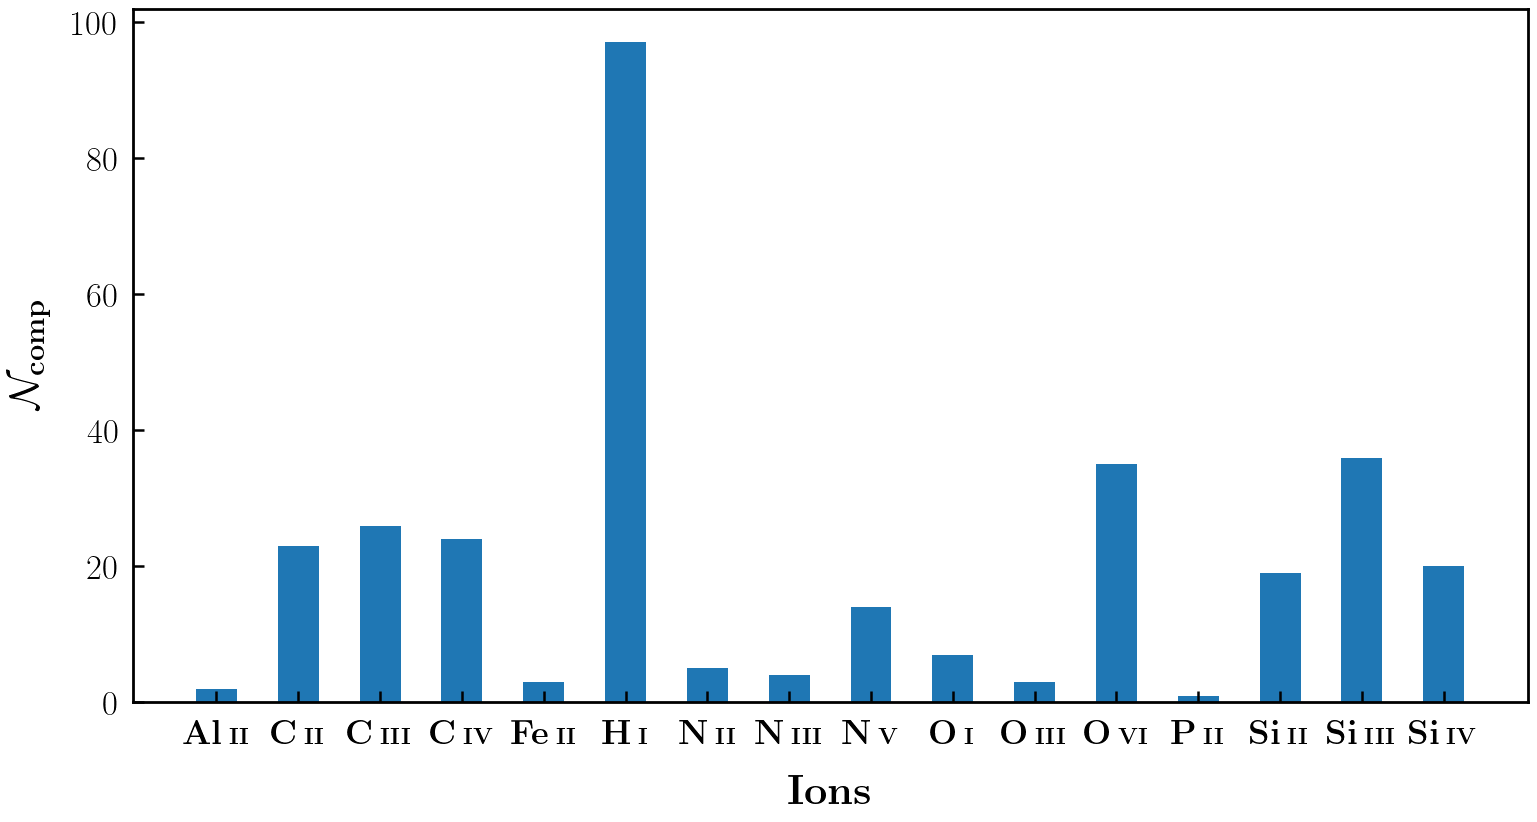
\includegraphics[width=\linewidth]{Figures/ion-component.png}
    \caption{No. of components identified for \ion{H}{i} and different metal ions.}
    \label{fig:comp-distribution}
\end{figure}

\begin{figure}
    \centering
    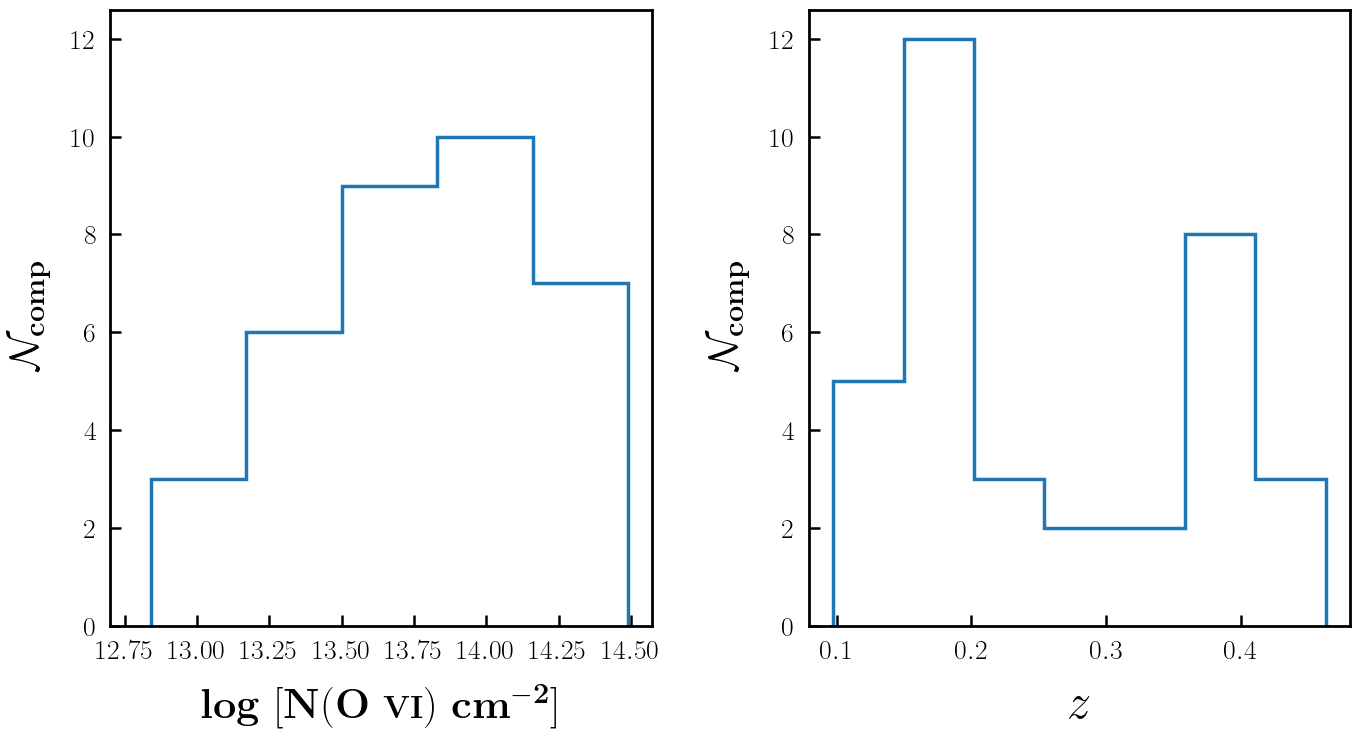
\includegraphics[width=\linewidth]{Figures/OVI_distribution_survey.png}
    \caption{No. of components identified for \ion{H}{i} and different metal ions.}
    \label{fig:comp-distribution}
\end{figure}

\begin{figure}
    \centering
    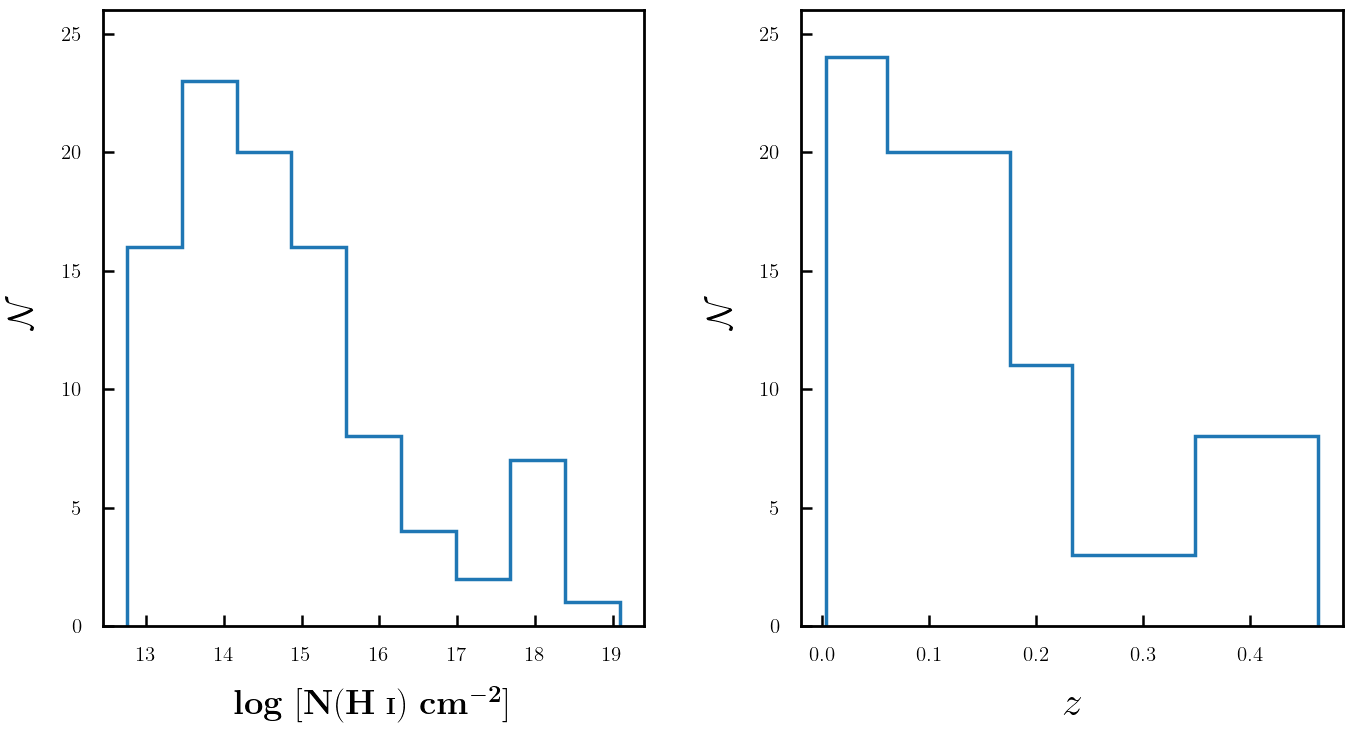
\includegraphics[width=\linewidth]{Figures/HI_distribution_survey.png}
    \caption{Left panel - distribution of \ion{H}{i} column densities, Right panel - distribution of redshift of \ion{H}{i} components}
    \label{fig:HI_distribution}
\end{figure}

\subsection{Ionisation modelling}





\section{Survey so far} \label{sec:OVI-BLA}

Out of the 28 BLA candidate systems identified as described in section \ref{sec:BLA-candidates}, we first focus on a subset of these systems which have \ion{O}{vi} absorption, as \ion{O}{vi} is a good tracer of WHIM. We have 16 such absorber systems. We begin the survey with these 16 systems. First step of the survey is to fit the Voigt profiles to all the lines identified in these systems. Currently, we have completed the preliminary fitting of these 16 absorber systems. The system plots of all these 16 systems are given in appendix \ref{ap:system-plots}.

